\documentclass[11pt]{article}
\usepackage[a4paper,margin=1in]{geometry}
\usepackage{amsmath}
\usepackage{graphicx}
\usepackage{xcolor}
\usepackage{booktabs}
\usepackage{parskip}
\usepackage{enumitem}
\usepackage[hidelinks]{hyperref}

\graphicspath{{../drawings/}{../modeling/}}
\definecolor{ink}{HTML}{1B2430}
\definecolor{acc}{HTML}{B3122B}
\setlist{nosep,leftmargin=1.4em}

\newcommand{\fig}[3]{\begin{figure}[ht]\centering\includegraphics[width=#2\textwidth]{#1}\caption{#3}\end{figure}}

\title{\textbf{\textcolor{ink}{Formula Zynerji}}\\[2pt]
\large A Blockchain-Based, Mechanism-Design Redesign of Formula~1 for Meritocracy}
\author{Zynerji \quad\textperiodcentered\quad \texttt{cknopp@gmail.com}}
\date{Draft v0.5 \textperiodcentered\ 2026 \textperiodcentered\ CC BY-SA 4.0}

\begin{document}
\maketitle

\begin{abstract}
\noindent Formula~Zynerji re-derives the Formula~1 rulebook from a single objective --- \textbf{meritocracy} --- using game theory and seventy years of how teams have actually behaved. Its spine is a \textbf{blockchain}: every part that runs on a car must have its full design (CAD/FEA/CFD) uploaded to an immutable ledger, and only on-chain parts are legal. Forced disclosure converts R\&D from a private secret into a shared club good, which collapses the spending war and lets the field \emph{self-balance by copying} --- with no development tokens, no auction, and no Balance of Performance. A mandatory minimum-spend floor forces continuous innovation; the resulting shared, race-validated engineering corpus is sold to outside industry to fund the sport and the prize money. The car is a deliberate kitbash of historical F1 eras around a distinctive 2.5\,L two-stroke uniflow diesel. This paper presents the thesis, the mechanisms (catalogued M1--M13), the car, the competition format, and the economic model that pins the two keystone numbers.
\end{abstract}

\section{Thesis: the championship as a measurement instrument}
A season is an \emph{estimator} of an unobservable quantity --- true competitive merit (car $+$ team $+$ driver). The standings are the estimate; meritocracy is the program of minimising the gap between them:
\[ \text{Standings} \;=\; \text{Merit} \;+\; \text{Luck} \;+\; \text{Budget-bias} \;+\; \text{Gaming-bias}. \]
Every rule is an intervention on one of those error terms, and is judged by one test: does it make the finishing order track merit more closely? Formula~1's instinct has been to remove danger and cost by \emph{banning} innovations (flat floors 1983, the turbo ban 1989, the electronic-aid ban 1994). Formula~Zynerji keeps the engineering freedom of the 1966--1982 open era but contains its two killers --- danger and runaway cost --- with a tight \emph{box} (a non-negotiable safety floor, a single energy/power pinch-point, and a self-balancing economy) rather than prescriptive bans. The design razors and the full mechanism catalogue (M1--M13) live in the project's \texttt{mechanism-design} document.

\section{The spine: forced on-chain disclosure (M10/M11)}
Every run part's complete design record is committed to an immutable, timestamped chain by the start of each event; \textbf{only on-chain parts are legal}, so scrutineering reduces to a hash check and a secret or back-dated part is structurally impossible. The economic consequence is the point: an innovation, once raced, is visible and copyable, so the value of any one advantage is capped at the head-start it buys. No team will spend millions for an edge that arms its rivals within a weekend --- equilibrium R\&D spend collapses, and the contest shifts from \emph{hiding the biggest secret} to \emph{innovating fastest and integrating best}. The innovator's reward is the transient head-start (you are fast first, and score points, before rivals can manufacture a copy) plus reputational recognition on a published Innovation Index. There are no tokens and no bounty.

\fig{blockchain_economy}{0.92}{The blockchain spine: on-chain legality (A), the self-balancing economy (B), and the revenue streams that fund the sport (C).}

\section{The self-balancing economy and its revenue}
Because forced disclosure makes copying free, the field balances itself: any advantage is copied away (the field compresses), the championship pulls every team toward the best on-chain parts, and re-leading demands fresh innovation. This removed the need for the artificial balancing machinery of earlier drafts --- development tokens, a development auction, and a success handicap are all \textbf{deleted}. The only economic levers are a hard, money-neutral \textbf{cap} and a mandatory minimum-spend \textbf{floor}. The floor is the keystone: a token-free copy economy has exactly one bad equilibrium --- everyone copies, nobody innovates --- and the floor forecloses it by forcing every team to do original development.

The shared corpus is also a \textbf{product}. Forced disclosure makes the chain a continuously-growing, cross-validated, race-proven engineering dataset, sold through tiered access: competitors get it free (disclosure is how they compete); journalists pay a media tier; and \textbf{non-competing industry} --- aerospace, defence, automotive and energy firms such as Boeing and Lockheed --- license the deep CAD/FEA/CFD, materials and control data for their own R\&D at a premium. This is the largest stream, and it funds the series' operations, the \textbf{prize money} for the four championships, and a redistribution toward smaller teams. Richer innovation makes the corpus more valuable, which grows the prize fund --- a further reason to innovate.

\section{The car: an era kitbash}
The car deliberately ports specific historical F1 regulation sets: \textbf{2026} wings, floor, tyres and safety; \textbf{2021} hydraulically-interconnected suspension; a \textbf{2013} 7-speed gearbox; and \textbf{2008} chassis dimensions and body rules. A 3300\,mm wheelbase, 1800\,mm width and $\sim$605\,kg minimum mass give a planted but ferociously powerful machine. Aero is disciplined not by ever-more-prescriptive geometry but by \emph{dirty-air externality pricing} (M4): each car's wake is measured, and a clean-wake car is granted a larger design-stage downforce allowance --- so close racing and overtaking happen on merit, and there is no DRS.

\fig{car_ga}{0.98}{Car general arrangement (side / plan / front) with the dimension set.}
\fig{car_3d}{0.98}{Parametric 3D general arrangement (CadQuery), exported to STEP.}

\section{The powertrain: a 2.5\,L two-stroke uniflow diesel}
The engine is a 2.5\,litre inline-five, two-stroke, uniflow-scavenged compression-ignition (diesel) unit on a JP-8-class synthetic e-kerosene, force-fed by a mechanical screw (Lysholm) supercharger, with no traction hybrid. Uniflow scavenging --- fresh charge in through liner ports at the bottom, exhaust out through poppet valves in the head --- is the most efficient two-stroke method and underpins the high BMEP. At 26\,bar BMEP and 7000\,rpm it makes $\sim$758\,kW ($\sim$1015\,hp) and $\sim$1035\,N\,m; at the 605\,kg minimum that is $\sim$1.25\,kW/kg, turbo-era-F1 power-to-weight. Exhaust tuning is by an electronically-controlled variable-length manifold (set-and-run): an automated \emph{engine} optimisation, not a driving aid.

\fig{engine_uniflow}{0.98}{The 2.5\,L I5 two-stroke uniflow diesel: cylinder cross-section and gas-path.}

\section{Driver-skill primacy and the vectoring differential}
The governing electronics principle is \emph{automate the engine, never the driving}: live manual driver inputs are encouraged; automated engine-output optimisation is permitted but locked before the race; automated car-control aids (traction control, ABS, closed-loop vectoring) are banned. The rear differential is a \textbf{driver-vectored} twin wet-clutch unit (GKN Twinster-type): two steering-wheel triggers set the percentage lockup of each side's clutch in real time. It is legal precisely because it is \emph{open-loop} --- the trigger-to-clamp map is fixed, declared and on-chain, and the safety ECU adds no sensor feedback --- which is what distinguishes it from banned automated vectoring.

\fig{diff_schematic}{0.95}{The driver-vectored twin wet-clutch differential and its open-loop control law.}

\section{The competition: a merit estimator}
The competition is tuned for signal-to-noise. The points curve scores \emph{all} classified finishers on a convex 40$\rightarrow$1 scale, so mid-grid merit is measured rather than rounded to zero. The Drivers' title is complemented by an advisory \textbf{Driver-Merit Index}: a hierarchical Bayesian model that separates a car effect from a driver effect using teammate comparisons (identical machinery), tied onto one scale and reproducible from on-chain data --- revealing the best driver net of machinery without corrupting team behaviour. A signature rule replaces blue flags with \emph{lapping elimination}: a backmarker may fight, but if it is lapped by the leader it is black-flagged out, and the leader scores a point. Because only the leader can ever lap a car first, the rule cleanly removes lapped-traffic interference --- every car still running is on the lead lap.

\section{Safety: the invariant}
Safety is the one part of the formula that is never an objective to be optimised and never traded: a non-negotiable, outcome-based floor (crash-test pass criteria, a halo-equivalent cockpit structure, homologated energy storage, driver equipment, and circuit/medical/spectator-separation minima written at the ruleset level). Engineering freedom and rigid safety standards are orthogonal --- one can run a tightly tuned competition while mandating exact crash-test outcomes.

\section{Economic model: pinning the cap and the floor}
The two keystone numbers were set from an explicit model rather than guessed.
\textbf{Cap.} A bottom-up cost build for a lean, shared-design program puts a competent entry at $\sim$\$67\,M and a running-cost floor at $\sim$\$56\,M, so a \textbf{\$75\,M} cap is $\sim$1.1$\times$ competent --- a genuinely tight constraint with real development headroom, while still binding the teams who would outspend it.
\textbf{Floor.} An innovate-versus-copy game shows that with no floor, teams self-select only $\sim$13\% original-R\&D (the public-goods under-provision that justifies the floor). Vitality rises monotonically with the floor at no cost to merit-correlation or field-compression, so the floor is a pure vitality-versus-affordability lever; and because the running-cost floor is $\sim$75\% of the cap, the floor must sit above it to bite --- hence \textbf{80\% of the cap}.

\begin{figure}[ht]\centering
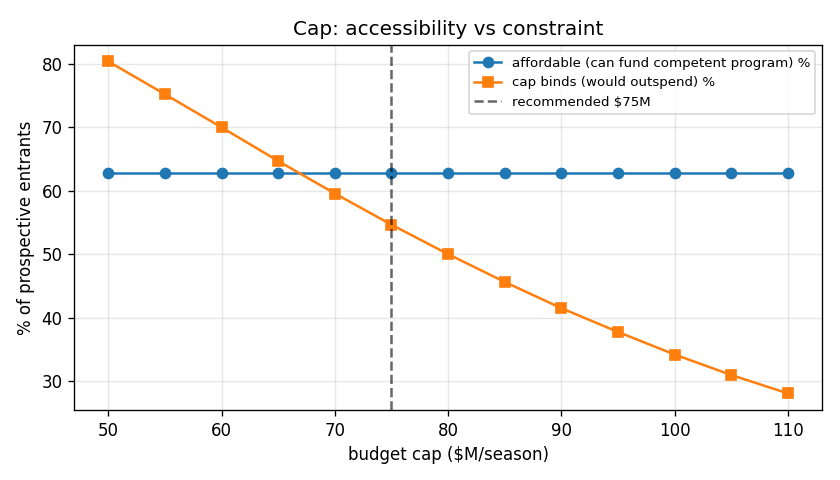
\includegraphics[width=0.49\textwidth]{cap_accessibility.png}\hfill
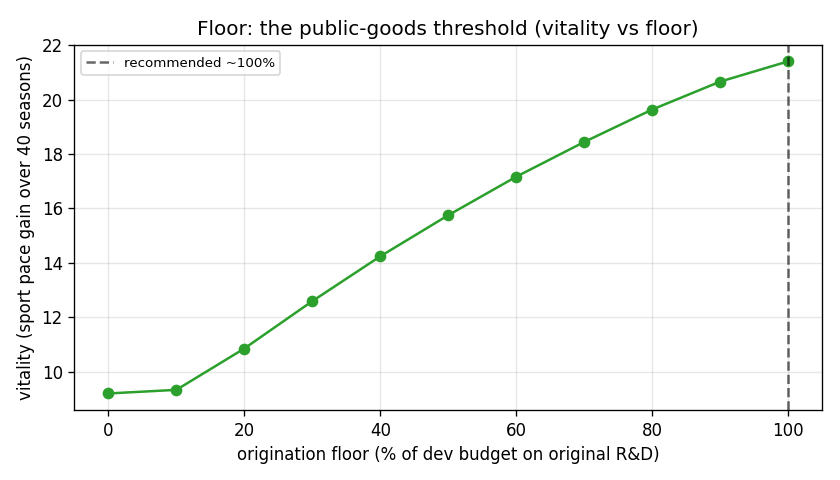
\includegraphics[width=0.49\textwidth]{floor_sweep.png}
\caption{Left: cap accessibility versus constraint. Right: the floor as the public-goods threshold (vitality versus the origination floor).}
\end{figure}

\section{Conclusion}
Formula~Zynerji is, in one line, the engineering freedom of 1970s Formula~1 wearing 2020s safety and a blockchain economy. By forcing disclosure, capping money, mandating a contribution floor, pricing the dirty-air externality, keeping the driving manual, and measuring driver merit explicitly, it makes the championship a faithful instrument for merit --- and turns the sport's own shared R\&D into the revenue that funds it.

\vspace{1em}\noindent\small\textit{The full regulations (technical, sporting, safety, financial), the mechanism catalogue, the economic model, and the figure sources are openly available at \texttt{github.com/Zynerji/FormulaZynerji}.}

\end{document}
